% Lensing, Fermat's principle and potential. Time delay surface.



\begin{figure*}
% \centering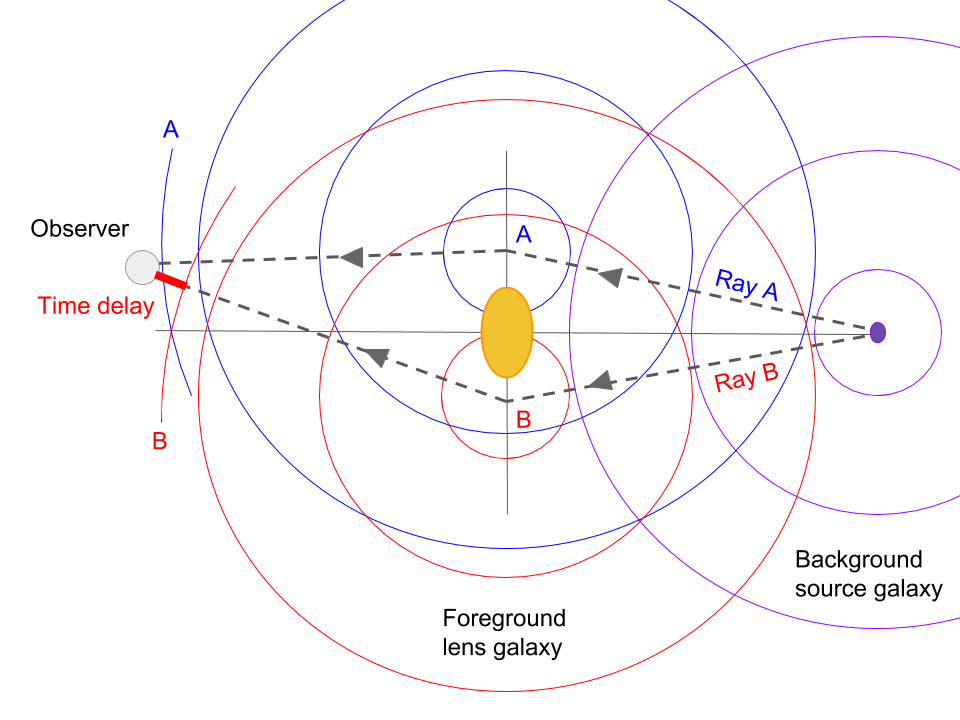
\includegraphics[width=0.96\textwidth]{figures/wavefront-schematic.pdf}
\caption{Schematic diagram, adapted from \citep{TreuAndEllis2015},
illustrating the origin of the gravitational time delay. The small
magnitude of the fractional  time delay (typically $\sim10$~days out of
$10^{12}$ days light travel time) is commensurate with the square of the
deflection angle (typically $\sim1$~arcsecond, or $\sim5\times10^{-6}$
radians).}
\label{fig:lineofsightcartoon}
\end{figure*}

% Time delay distance.

% Importance of mass distribution in lens.

% Model (mass-sheet) degeneracy and its generalizations

% Importance of mass along the line sight - the universe is not Friedmann Lemaitre Robertson Walker.


\begin{figure*}
% \centering\includegraphics[width=0.96\textwidth]{figures/line-of-sight-cartoon.pdf}
\caption{Cartoon illustration of line of sight effects in time delay
lens cosmography. Structures both within and outside the main lens
plane provide weak deflections to the light rays, affecting both the
image positions and time delays.} \label{fig:lineofsightcartoon}
\end{figure*}
